\documentclass[]{beamer}
\mode<presentation>{
  %% \usetheme[compress]{Berlin}
}
%% packages
\usepackage{zhspacing}
\zhspacing
\usepackage{graphics}
\usepackage{subfigure}
\usepackage{listings}
\lstset{
  basicstyle=\ttfamily\tiny,
  numbers=left
}
\usepackage{tabularx}
\usepackage{booktabs}
%% meta info
\title{Breadth-First Search on Multicore Architecture}
\subtitle{Special Topic on BFS (1)}
\author[SuXing~pysuxing@gmail.com]{SuXing}
\institute{TOW}
\date{\today}

\setbeamercolor{footcolor}{fg=blue,bg=white} % 设置字体和背景颜色
\setbeamertemplate{footline}{%
  \leavevmode%
  \hbox{%
    \begin{beamercolorbox}[wd=.126\paperwidth,ht=2.25ex,dp=1ex,right]{footcolor}%      
       \insertframenumber{} / \inserttotalframenumber\hspace*{5ex}
    \end{beamercolorbox}}%
  \vskip0pt%
}

%% slides
\begin{document}
\bibliographystyle{plain} 
\setlength{\parindent}{0pt}

\frame{\titlepage}
\frame{\tableofcontents[hideallsubsections]}

\section{Background}
\frame{\tableofcontents[currentsection]}

\subsection{Breadth-First Search}
\frame{\tableofcontents[currentsection, currentsubsection]}

\begin{frame}
  \frametitle{Importance of BFS}
  \begin{itemize}
    \item Graph analysis's becoming more and more important\\
      e.g. computational sciences, social network analysis, security, and business analytics
    \item BFS is a basic kernel in building large-scale parallel graph algorithms\\
      e.g. between-centrality(BC), strong connected components(SCC), single source shortest path(SSSP)
  \end{itemize}
\end{frame}

\begin{frame}
  \frametitle{Challenging Issues}
  Some challenge issues rise in general graph algorithms, among which the most highlighted ones are
  \begin{itemize}
    \item irregular memory access patterns (bad locality)
    \item unbalanced load distribution
  \end{itemize}
  BFS as an active example, a vertex can has arbitary vertex as its neighbor (issue \#1), and can has
  arbitary number of neighbors (issue \#2).
\end{frame}

\subsection{Modern Multicore Architecture}
\frame{\tableofcontents[currentsection, currentsubsection]}

\begin{frame}
  \frametitle{Multi-socket Architecture}
  As number of cores increases in a single processor, cores are organized in multiple sockets.
  Sockets are connected with intra-processor networks, with their caches synchronized by coherence protocols
  \begin{figure}
    \centering
    \subfigure{
      \begin{minipage}[t]{0.45\textwidth}
        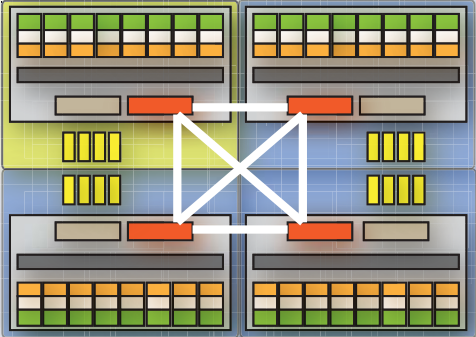
\includegraphics[width=\textwidth]{figures/nehalem-ex-4skts}
        \caption{Nehalem EX (4X)}
      \end{minipage}
    }
    \subfigure{
      \begin{minipage}[t]{0.45\textwidth}
        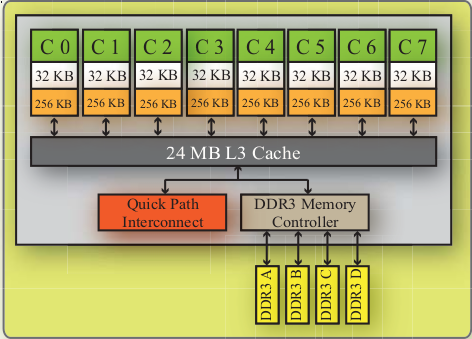
\includegraphics[width=\textwidth]{figures/nehalem-ex}
        \caption{Nehalem EX}
      \end{minipage}
    }
  \end{figure}
\end{frame}

\begin{frame}
  \frametitle{Best Performance Guidelines}
  Two general approaches to achieve best performance in HPC are fully utilizing
  \begin{itemize}
    \item computational hardware
    \item memory and interconnect bandwidth
  \end{itemize}
  For memory intensive problems with inherent low computation-communication ratio
  (e.g. BFS and other graph algorithms),
  achieving high memory bandwidth deserves the most effort
\end{frame}

\begin{frame}
  \frametitle{Achieving high bandwidth on SMPs}
  Keys to high bandwidth on SMPs
  \begin{itemize}
    \item utilizing cache
    \item hiding memory latency
    \item decreasing inter-socket cache coherence overhead
  \end{itemize}
  \begin{figure}
    \centering
    \subfigure{
      \begin{minipage}[t]{0.45\textwidth}
        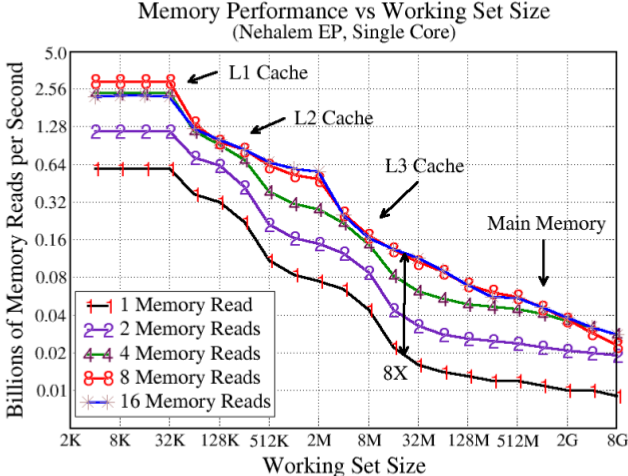
\includegraphics[width=\textwidth]{figures/cache-utilization}
        \caption{single core read-only access}
      \end{minipage}
    }
    \subfigure{
      \begin{minipage}[t]{0.45\textwidth}
        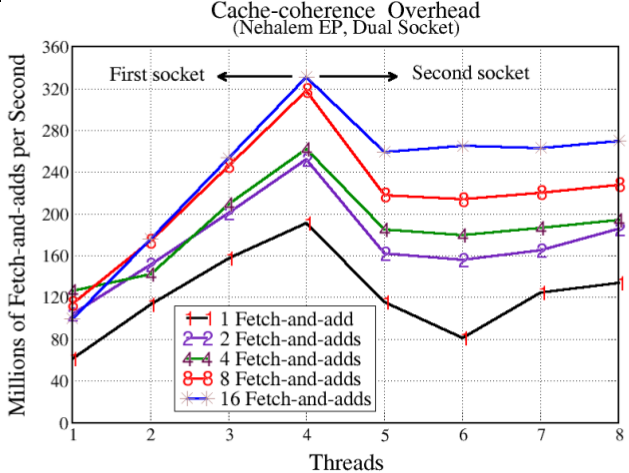
\includegraphics[width=\textwidth]{figures/inter-socket-coherence}
        \caption{multi-threaded read-write access}
      \end{minipage}
    }
  \end{figure}
\end{frame}

\section{Algorithm}
\frame{\tableofcontents[currentsection]}

\begin{frame}
  \frametitle{High-Level Overview}
  \begin{figure}
    \centering
    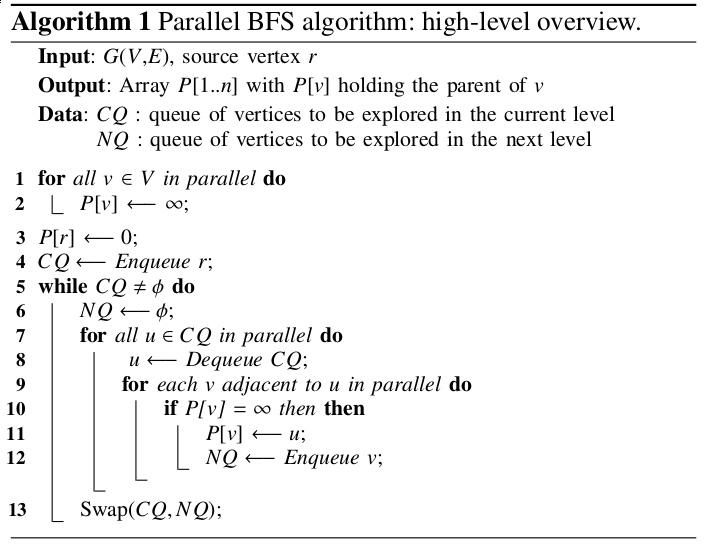
\includegraphics[width=.8\textwidth]{figures/bfs-serial}
  \end{figure}
\end{frame}

\begin{frame}
  \frametitle{Representation of BFS Result}
  Typically, BFS Result could have two forms of representation
  \begin{itemize}
    \item Parent Array (P)
    \item Depth Array (D)
  \end{itemize}
  An implementation could use either or both. e.g. The graph500 benchmark
  uses the Parent Array form
\end{frame}

\begin{frame}
  \frametitle{Parallelization}
  \begin{itemize}
    \item The parallelism lies in the for loop on line 7, all vertices in CQ
      are partitioned to simultaneous worker threads
    \item CQ, NQ and P are shared amoung all threads, so write access should be
      protected (may be relaxed)
  \end{itemize}
  \begin{figure}
    \centering
    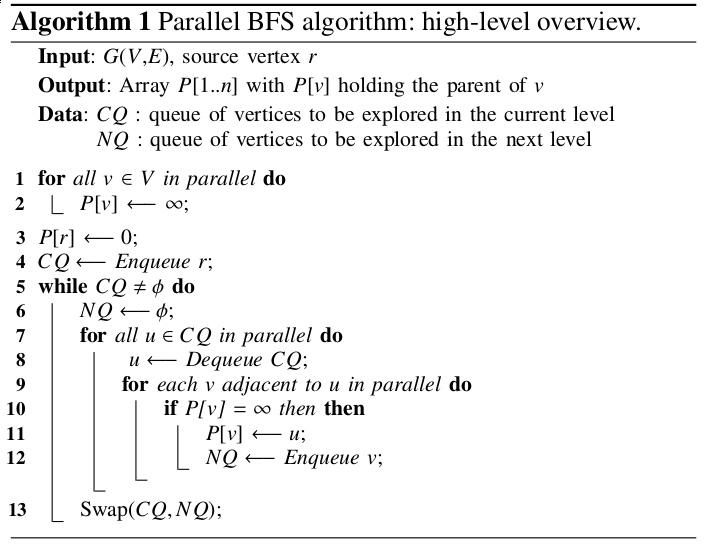
\includegraphics[width=.5\textwidth]{figures/bfs-serial}
  \end{figure}
\end{frame}

\section{Implementation}
\frame{\tableofcontents[currentsection]}

\begin{frame}
  \frametitle{Proposed Implementation Techniques}
  Here we show implementation techniques proposed by two recent papers
  \begin{itemize}
    \item Scalable Graph Exploration on Multicore Processors\cite{Agarwal2010} (SC'10)
    \item Fast and Efficient Graph Traversal Algorithm for CPUs Maximizing Single-Node
      Efficiency\cite{Chhugani2012} (IPDPS'12)
  \end{itemize}
  We'll refer them as SC'10 and IPDPS'12 respectively
\end{frame}

\subsection{Approaches by SC'10}
\frame{\tableofcontents[currentsection, currentsubsection]}

\begin{frame}
  \frametitle{SC'10 Outline}
  SC'10 proposed several implementation techniques
  \begin{itemize}
    \item caches utilization
    \item elimating lock overhead
    \item optimizing inter-socket communication
  \end{itemize}
\end{frame}

\begin{frame}
  \frametitle{Cache Utilization}
  \begin{columns}
    \begin{column}{.5\textwidth}
      \begin{itemize}
        \item Line 4, 13, 15\\
          Use a more cache-efficient data structure, bitmap, to query if a vertex is visted instead of P(D)
        \item Line 17\\
          But parts of P(D) still need be fetch into and evict from cache while being updated.
      \end{itemize}
    \end{column}
    \begin{column}{.5\textwidth}
      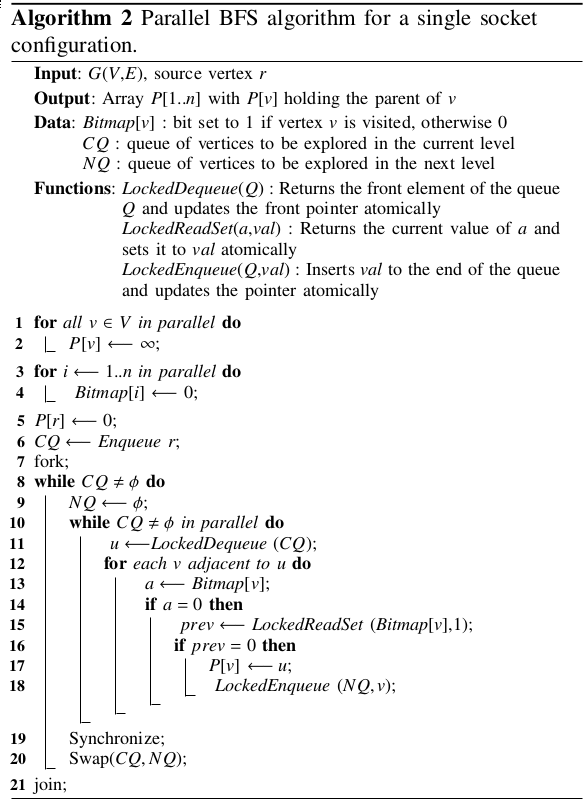
\includegraphics[width=\textwidth]{figures/sc10-algo2}
    \end{column}
  \end{columns}
\end{frame}

\begin{frame}
  \frametitle{Elimating lock overhead}
  \begin{columns}
    \begin{column}{.5\textwidth}
      \begin{itemize}
        \item Line 13, 15\\
          Doubled checking of the visited bitmap, which make a considerable
          decreasement in number atomic operations
      \end{itemize}
      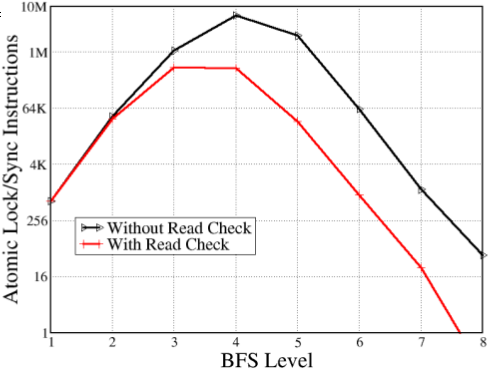
\includegraphics[width=\textwidth]{figures/sc10-lock-elimation}
    \end{column}
    \begin{column}{.5\textwidth}
      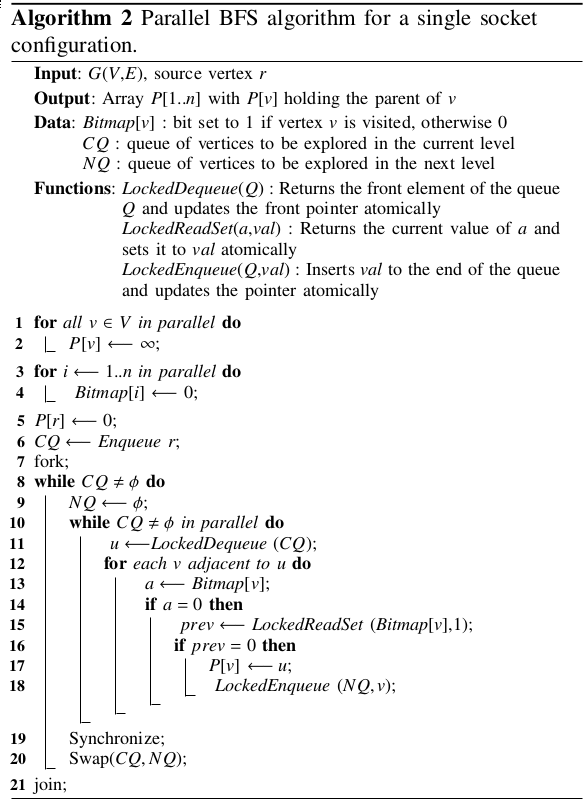
\includegraphics[width=\textwidth]{figures/sc10-algo2}
    \end{column}
  \end{columns}
\end{frame}

\begin{frame}
  \frametitle{Optimizing inter-socket communication}
  \begin{columns}
    \begin{column}{.55\textwidth}
      \begin{itemize}
        \item A two phase updation of shared data structures.
          In phase 1, a socket only updates its own part of shared data and
          buffer newly discovered vertices owned by other sockets (Line 18-24).
          In phase 2, all buffered vertices are processed (Line 28-35)
        \item SQ is a low overlead lock-free queue for inter-socket communication (Line 26, 29)
        \item Use batching when inserting into and remove from SQ to elimate contention (Line 26, 29)
      \end{itemize}
    \end{column}
    \begin{column}{.45\textwidth}
      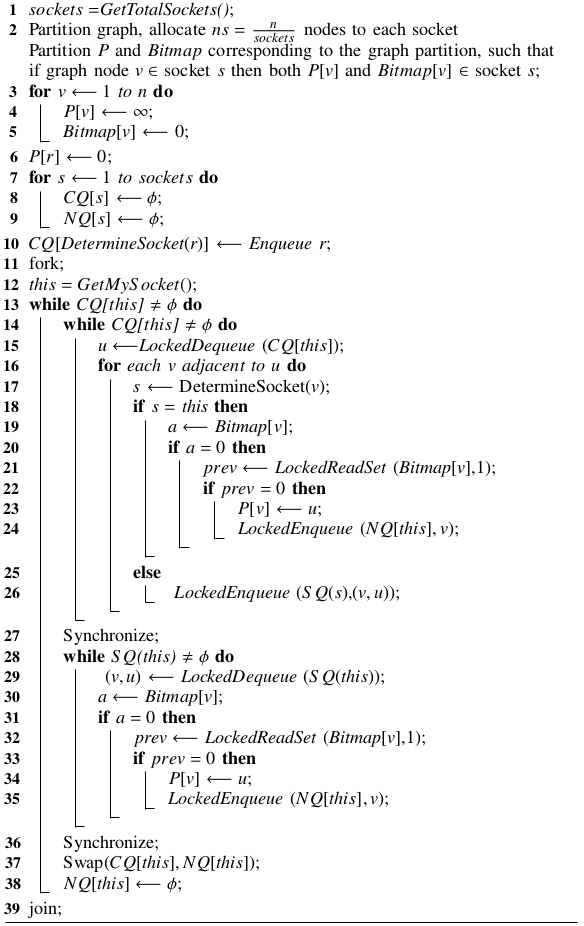
\includegraphics[width=\textwidth]{figures/sc10-algo3}
    \end{column}
  \end{columns}
\end{frame}

\begin{frame}
  \frametitle{Performance Evaluation}
  \begin{figure}
    \centering
    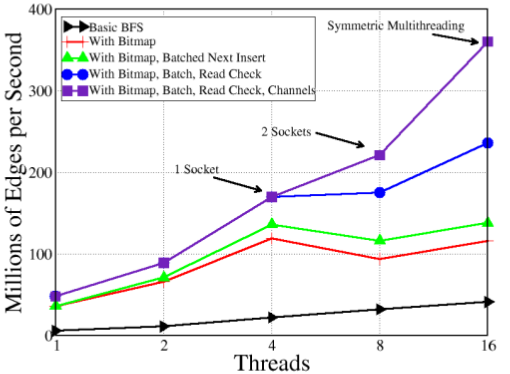
\includegraphics[width=.5\textwidth]{figures/sc10-evaluation}
    \caption{Impact of various optimizations}
  \end{figure}
\end{frame}

\subsection{Approaches by IPDPS'12}
\frame{\tableofcontents[currentsection, currentsubsection]}

\begin{frame}
  \frametitle{IPDPS'12 Outline}
  IPDPS'12 proposed some enhancement to SC'10, along with a few more optimizations
  \begin{itemize}
    \item more aggressive cache utilization
    \item totally lock- and atomic-free updates of shared data structures
    \item inter-socket load-balancing techniques
  \end{itemize}
\end{frame}

\begin{frame}
  \frametitle{Cache Utilization}
  IPDPS'12 supports extremely large graphs by partition visited bitmap (VIS) among sockets.
  So only a chunk of VIS stays in sockets' LLC
  \begin{block}{Motivation}
  The bitmap approache proposed by SC'10 cannot handle extremely large graphs whose
  VIS may be too large to fit into LLC, and performance would decrease
  in such cases
  \end{block}
  %% figure here
  The proper chunck size may be C/4 or C/2 where C is the LLC size
\end{frame}

\begin{frame}
  \frametitle{Elimating lock overhead}
  IPDPS'12 do not use any lock or atomic operations when updating VIS or D(P)
  \begin{block}{Insight}
    Certain write protection can be relaxed when preserving correctness
  \end{block}
  \begin{figure}
    \centering
    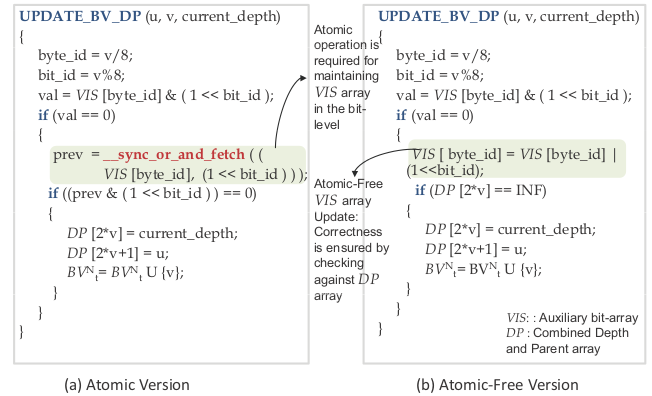
\includegraphics[width=.6\textwidth]{figures/ipdps12-atomic-free}
    %% \caption{Atomic and atomic-free updating method comparision}
  \end{figure}
  NOTE: Simultaneous updation to VIS or D(P) may occure due to lockless access, which
  is practically a rare case (0.2\% inspected)
\end{frame}

\begin{frame}
  \frametitle{Inter-socket Load-Balancing}
  IPDPS'12 adopes a balanced work partitioning method, with acceptable inter-socket communication.
  \begin{block}{Motivation}
  SC'10 2-phase approache effectively decrease inter-socket communication, but the straightforward
  partition method may lead to poor load-balancing, especially for graphs with non-uniform degree
  distribution
  \end{block}
  We'll make it clear by an example
\end{frame}

\begin{frame}
  \frametitle{Inter-socket Load-Balancing Example}
  Assume a configuration
  \begin{itemize}
    \item CPU has 4 sockets
    \item VIS is partitioned to five chunks
  \end{itemize}
  \begin{figure}
    \centering
    \includegraphics[width=\textwidth]{figures/ipdps12-load-banlancing}
  \end{figure}
\end{frame}

\begin{frame}
  \frametitle{Performance Evaluation}
  \begin{figure}
    \centering
    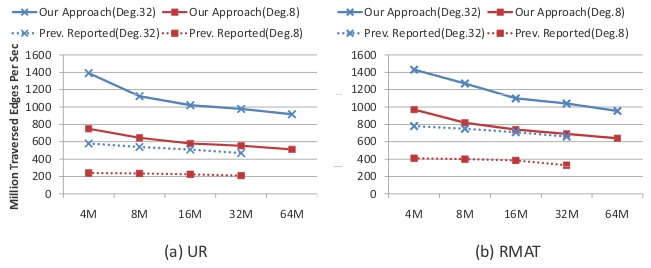
\includegraphics[width=.8\textwidth]{figures/ipdps12-evaluation}
    \caption{Performance compared to SC'10}
  \end{figure}
\end{frame}

\section{Summary}
\frame{\tableofcontents[currentsection]}

\begin{frame}
  \frametitle{Summary}
  \begin{itemize}
    \item Modern multi-socket processor architecture
    \item Parallel BFS algorithm
    \item BFS implementation techniques on SMP proposed by two recent papers
      \begin{itemize}
        \item Fully utilizing cache to achieve high bandwidth
        \item Elimating lock and atomic operations
        \item Optimizing inter-socket communication
        \item Inter-socket load-balancing
      \end{itemize}
  \end{itemize}
\end{frame}

\begin{frame}
  \frametitle{References}
  \bibliography{refs.bib}
\end{frame}

\frame{\centerline{\Huge Q\&A}}

\end{document}
